\hypertarget{group__group26}{
\chapter{Functional Overview}
\label{group__group26}
}

\begin{flushleft}
OpenClovis ASP is a distributed system with many redundant servers. These servers interact with each other to provide the required services to the 
applications. The servers can be individual processes executing in separate address spaces. The interaction is possible, if an efficient and effective 
means of communication exists between these servers. Remote Procedure Call (RPC) mechanism is often used to enable communication between processes 
existing in different address spaces. 
\par
The OpenClovis Remote Method Dispatch (RMD), implements RPC semantics using synchronous and asynchronous methods. RMD transparently 
invokes methods exported by various objects. The objects on which a method is invoked can exist locally or on a remote blade. RMD supports both 
synchronous and asynchronous calls. The latter includes calls with and without return information. Signature check and version check is performed at 
run-time as part of the RMD call. At-most-once semantics ensures that the request is never executed more than once by the service provider. 
\par
RMD calls can fail due to reasons beyond the semantics of the operation. Some of the possible causes include link failure, component failure, and 
communication overload. These errors are handled by the RMD and the error handlers registered by the application.

\chapter{Service Model}
\section{Usage Model}
When an object requires the service of another object, it needs to call that particular object. This call is trapped by the RPC mechanism, which sends the
parameters of the call to the destination object across the network. The RPC mechanism receives the parameters and calls the relevant function residing 
on the destination server. This function executes in the address space of the destination and returns the control (and parameters) to the RPC mechanism, 
on the server at the destination. 
This return result is returned to the RPC mechanism at the client (caller). The caller's RPC returns the result to the caller, that continues as if it 
returned from a normal (local) function call.
The RMD is built on the same mechanism as the RPC. The RMD mechanism uses the OpenClovis IOC protocol as the transport layer for communication and
enables communication between components (processes). IOC is responsible for the transportation of packets across servers. A component is the unit of 
execution of ASP and it is equivalent to a process in many ways.
\begin{figure}[htp]
\centering
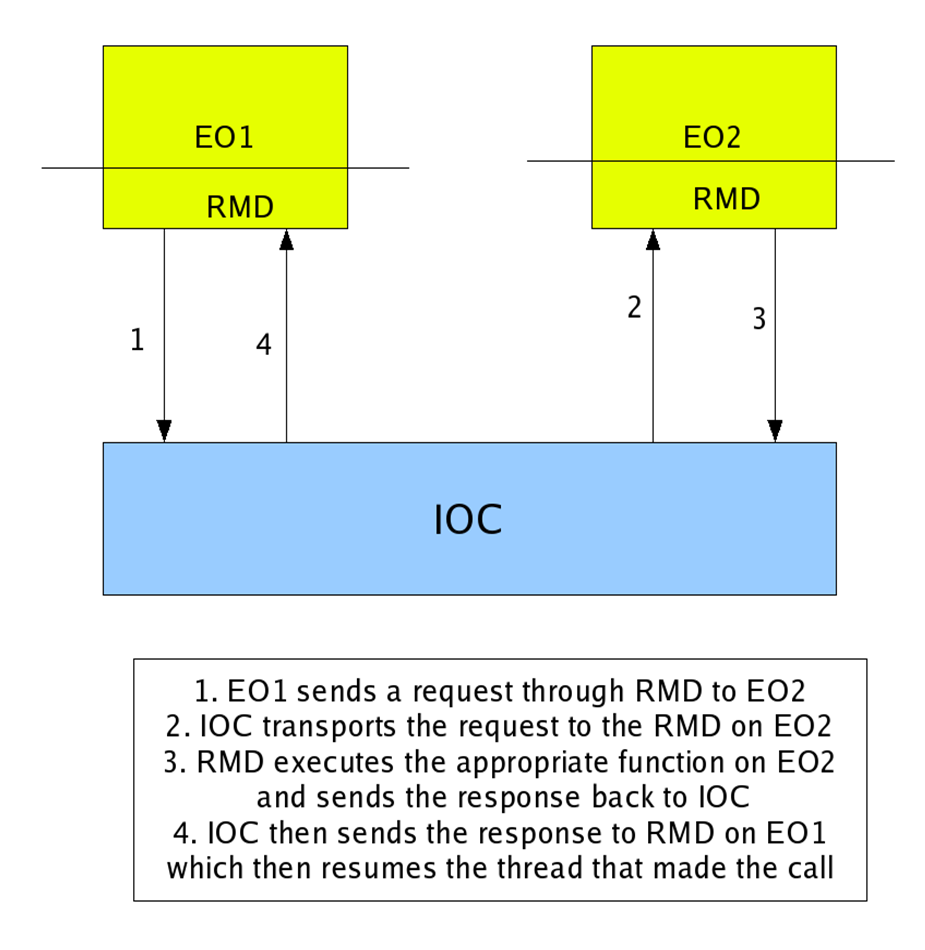
\includegraphics{rmd.png}
\caption{Communication Based on RMD}
\end{figure}


\chapter{Service APIs}



\section{Type Definitions}

\subsection{ClRmdOptionsT}
\index{clRmdWithMsg@{clRmdWithMsg}}
\begin{tabbing}
xx\=xx\=xx\=xx\=xx\=xx\=xx\=xx\=xx\=\kill
\textit{typedef struct ClRmdOptions\{}\\
\>\>\>\>\textit{ClUint32T timeout;}\\
\>\>\>\>\textit{ClUint32T retries;}\\
\>\>\>\>\textit{ClUint8T priority;}\\
\>\>\>\>\textit{ClIocToBindHandleT transportHandle;}\\
\textit{\} ClRmdOptionsT;}\end{tabbing}
 The structure, {\tt{ClRmdOptionsT}}, is used to pass any optional parameters to RMD.
\begin{itemize}
\item
\textit{timeout} - Timeout value in milliseconds. It is the expected time of execution of the remote function in the order of the minimum resolution 
provided by the timer library. The values 1 or 0 indicate timeout forever.
\item
\textit{retries} - Maximum number of times you can retry after the first call, if a timeout has occurred.
\item
\textit{priority} - Priority value for the call. It is passed to the IOC without modification.
\item
\textit{transportHandle} - Transport handle obtained through {\tt{clIocBind()}} for an RMD call through the specified transport. 
\end{itemize}


\subsection{clRMDAsyncOptionsT}
\index{clRMDAsyncOptionsT@{clRMDAsyncOptionsT}}
\begin{tabbing}
xx\=xx\=xx\=xx\=xx\=xx\=xx\=xx\=xx\=\kill
\textit{typedef struct \{}\\
\>\>\>\>\textit{ClRmdAsyncCallbackT fpCallback;}\\
\>\>\>\>\textit{void *pCookie;}\\
\textit{\} clRMDAsyncOptions;}\end{tabbing}
\textit{typedef struct clRMDAsyncOptions ClRmdAsyncOptionsT;}
\newline
\newline
This structure, {\tt{clRMDAsyncOptions}}, is used to pass additional parameters to the {\tt{clRmdWithMsg()}} asynchronous call.
\begin{itemize}
\item
\textit{fpCallback} - Calling application's callback.
\item
\textit{pCookie} - Calling application's cookie.
\end{itemize}


\newpage

\section{Functional APIs}
\subsection{clRmdWithMsg}
\index{clRmdWithMsg@{clRmdWithMsg}}
\hypertarget{pagermd103}{}\paragraph{cl\-Rmd\-With\-Msg}\label{pagermd103}
\begin{Desc}
\item[Synopsis:]Invokes a remote function call when the parameters are passed as messages. \end{Desc}
\begin{Desc}
\item[Header File:]clRmdApi.h\end{Desc}
\begin{Desc}
\item[Syntax:]

\footnotesize\begin{verbatim}        ClRcT clRmdWithMsg(
                                ClIocAddressT        remoteObjAddr,
                                ClUint32T           funcId,
                                ClBufferHandleT    inMsgHdl,
                                ClBufferHandleT    outMsgHdl,
                                ClUint32T           flags,
                                ClRmdOptionsT*       pOptions,);
\end{verbatim}
\normalsize
\end{Desc}
\begin{Desc}
\item[Parameters:]
\begin{description}
\item[{\em remote\-Obj\-Addr:}]Address of the destination Object. 
\item[{\em func\-Id:}]Function ID of the function to be executed. 
\item[{\em in\-Msg\-Hdl:}]This parameter is created and freed by the calling application, if {\tt{CL\_\-RMD\_\-CALL\_\-NON\_\-PERSISTENT}} is not set. If
this flag is set, RMD frees the message. If this parameter is NULL, no value is passed to the remote end by the caller. 
\item[{\em out\-Msg\-Hdl:}]Created and freed by the caller. If it is NULL and {\tt{CL\_\-RMD\_\-CALL\_\-NEED\_\-REPLY}} flag is set, 
{\tt{CL\_\-RMD\_\-RC (CL\_\-ERR\_\-INVALID\_\-PARAM)}} is returned.
\item[{\em flags:}]Informs RMD if the call is a synchronous call or an asynchronous call. It also indicates if at-most-once semantics is required or not. 
\item[{\em options:}]Indicates the optional parameters such as priority, timeout, cookie, retries, and callback function. If it is NULL, default
values (priority and timeout) are taken.
\item[{\em pAsyncOptions:}]This is to be passed only if the call is an asynchronous call. Optional parameters such as cookies and callback 
functions can be passed in this parameter.
 \end{description}
\end{Desc}
\begin{Desc}
\item[Return values:]
\begin{description}
\item[{\em CL\_\-OK:}]The function executed successfully. 
\item[{\em CL\_\-RMD\_\-RC(CL\_\-ERR\_\-NO\_\-MEMORY):}]The system memory is not available.
\item[{\em CL\_\-RMD\_\-RC(CL\_\-ERR\_\-TIMEOUT):}]Reply to this call was not received in the specified time or an invalid IOC port ID is passed to the 
function.
\item[{\em CL\_\-RMD\_\-RC(CL\_\-ERR\_\-NULL\_\-PTR):}]{\tt{pOptions}} contains a NULL pointer.
\item[{\em CL\_\-RMD\_\-RC(CL\_\-INVALID\_\-PARAMETER):}]An invalid parameter is passed as a parameter to the function. A parameter is not set correctly.
\item[{\em CL\_\-EO\_\-ERR\_\-FUNC\_\-NOT\_\-REGISTERED:}]The requested function is not registered. 
\item[{\em CL\_\-EO\_\-ERR\_\-EO\_\-SUSPENDED:}]The remote component is in the suspended state.

\item[{\em CL\_\-RMD\_\-RC(CL\_\-ERR\_\-NOT\_\-INITIALIZED):}]RMD Library is not initialized. 
\item[{\em CL\_\-IOC\_\-RC(CL\_\-IOC\_\-ERR\_\-RECV\_\-UNBLOCKED):}]The receiver is unblocked.
\item[{\em CL\_\-IOC\_\-RC(CL\_\-IOC\_\-ERR\_\-HOST\_\-UNREACHABLE):}]{\tt{remoteObjAddr}} contains an invalid node address.

\item[{\em CL\_\-IOC\_\-RC(CL\_\-ERR\_\-NOT\_\-EXIST):}]An invalid logical address has been passed to this function.
\item[{\em CL\_\-RMD\_\-RC(CL\_\-ERR\_\-NOT\_\-IMPLEMENTED):}]This type of call is not supported.
        This function can also return some OS defined error codes. 

\end{description}
\end{Desc}
\begin{Desc}
\item[Description:]This function is used to invoke a remote function call. The following parameters are required:
\begin{itemize}
\item
Destination address ({\tt{ObjectId}}) where the function resides
\item
{\tt{functionId}} of the function to be invoked
\item
Input parameter in a message
\item
Output message to receive the reply
\item
Flags specific to RMD
\item
RMD options
\item
RMD asynchronous call options - For an asynchronous call, options such as priority, timeout value, retries, cookie, and callback function must be 
passed in the structure, {\tt{ClRmdAsyncOptions}}. 
\end{itemize}
All parameters are not mandatory for every call. For a synchronous call, cookie and callback functions
are not required. The remote function is identified by the remote object address and the function ID.

\end{Desc}
\begin{Desc}
\item[Library File:]lib\-Cl\-Rmd\end{Desc}
\begin{Desc}
\item[Related Function(s):]None \end{Desc}

\newpage

\subsection{clRmdLibInitialize}
\index{clRmdLibInitialize@{clRmdLibInitialize}}
\hypertarget{pagermd104}{}\paragraph{cl\-Rmd\-Lib\-Initialize}\label{pagermd104}
\begin{Desc}
\item[Synopsis:]Initializes the RMD library.\end{Desc}
\begin{Desc}
\item[Header File:]clRmdApi.h\end{Desc}
\begin{Desc}
\item[Syntax:]

\footnotesize\begin{verbatim}        ClRcT clRmdLibInitialize(void);
\end{verbatim}
\normalsize
\end{Desc}
\begin{Desc}
\item[Return Values:]
\begin{description}
\item[{\em CL\_\-OK:}]The function executed successfully. 
\item[{\em CL\_\-RMD\_\-RC(CL\_\-ERR\_\-NO\_\-MEMORY):}]System memory is not available.
\item[{\em CL\_\-RMD\_\-RC(CL\_\-ERR\_\-NOT\_\-INITIALIZED):}]RMD Library is not initialized. 
\end{description}
\end{Desc}
\begin{Desc}
\item[Description:]
This function initializes the RMD library with default values if the RMD library is not initialized as part of the configuration of the component. 
Before an RMD function can be used, this function must be executed.
\end{Desc}
\begin{Desc}
\item[Library File:]lib\-Cl\-Rmd\end{Desc}
\begin{Desc}
\item[Related Function(s):]\hyperlink{pagermd105}clRmdLibFinalize. \end{Desc}

\newpage
\subsection{clRmdLibFinalize}
\index{clRmdLibFinalize@{clRmdLibFinalize}}
\hypertarget{pagermd105}{}\paragraph{cl\-Rmd\-Lib\-Finalize}\label{pagermd105}
\begin{Desc}
\item[Synopsis:]Finalizes the RMD library.\end{Desc}
\begin{Desc}
\item[Header File:]clRmdApi.h\end{Desc}
\begin{Desc}
\item[Syntax:]

\footnotesize\begin{verbatim}        ClRcT clRmdLibFinalize(void);
\end{verbatim}
\normalsize
\end{Desc}
\begin{Desc}
\item[Return Values:]
\begin{description}
\item[{\em CL\_\-OK:}]The function executed successfully. 
\item[{\em CL\_\-RMD\_\-RC(CL\_\-ERR\_\-NO\_\-MEMORY):}]System memory is not available.
\item[{\em CL\_\-RMD\_\-RC(CL\_\-ERR\_\-NOT\_\-INITIALIZED):}]RMD Library is not initialized. 
\end{description}
\end{Desc}
\begin{Desc}
\item[Description:]
This function is used to free the resources acquired by the RMD library when the RMD library is initialized. It must be invoked typically during the 
system shutdown process or if the RMD library is not required.
\end{Desc}
\begin{Desc}
\item[Library File:]lib\-Cl\-Rmd\end{Desc}
\begin{Desc}
\item[Related Function(s):]\hyperlink{pagermd104}clRmdLibInitialize. \end{Desc}
\end{flushleft}